%!TEX root = /Users/dan/Documents/Thesis/Thesis.tex
% Appendix B

\chapter{Root System Diagrams}
\label{AppendixB}
\lhead{Appendix B. \emph{Root System Diagrams}}

\section{Dynkin Diagrams}

Short roots are identified by filled circles.

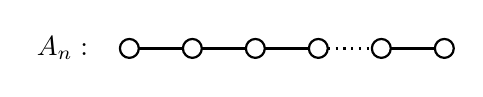
\begin{tikzpicture}[scale=.4]
\draw (-1,0) node[anchor=east]  {$A_n:$};
\foreach \x in {0,...,5}
\draw[xshift=\x cm, thick] (\x cm,0) circle (.3cm);
\draw[thick] (0.3 cm, 0) -- +(1.4 cm, 0);
\draw[thick] (2.3 cm, 0) -- +(1.4 cm, 0);
\draw[thick] (4.3 cm, 0) -- +(1.4 cm, 0);
\draw[dotted, thick] (6.3 cm, 0) -- +(1.4 cm, 0);
\draw[thick] (8.3 cm, 0) -- +(1.4 cm, 0);
\end{tikzpicture}

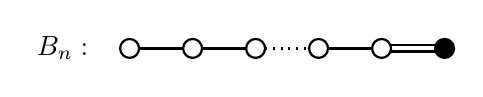
\begin{tikzpicture}[scale=.4]
\draw (-1,0) node[anchor=east]  {$B_n:$};
\foreach \x in {0,...,4}
\draw[xshift=\x cm, thick] (\x cm,0) circle (.3cm);
\draw[xshift=5 cm, thick, fill=black] (5 cm,0) circle (.3cm);
\draw[thick] (0.3 cm, 0) -- +(1.4 cm, 0);
\draw[thick] (2.3 cm, 0) -- +(1.4 cm, 0);
\draw[dotted,thick] (4.3 cm, 0) -- +(1.4 cm, 0);
\draw[thick] (6.3 cm, 0) -- +(1.4 cm, 0);
\draw[thick] (8.3 cm, 0.1) -- +(1.4 cm, 0);
\draw[thick] (8.3 cm, -0.1) -- +(1.4 cm, 0);
\end{tikzpicture}


\begin{tikzpicture}[scale=.4]
\draw (-1,0) node[anchor=east]  {$C_n:$};
\foreach \x in {0,...,4}
\draw[xshift=\x cm, thick, fill=black] (\x cm,0) circle (.3cm);
\draw[xshift=5 cm, thick] (5 cm,0) circle (.3cm);
\draw[thick] (0.3 cm, 0) -- +(1.4 cm, 0);
\draw[thick] (2.3 cm, 0) -- +(1.4 cm, 0);
\draw[dotted,thick] (4.3 cm, 0) -- +(1.4 cm, 0);
\draw[thick] (6.3 cm, 0) -- +(1.4 cm, 0);
\draw[thick] (8.3 cm, 0.1) -- +(1.4 cm, 0);
\draw[thick] (8.3 cm, -0.1) -- +(1.4 cm, 0);
\end{tikzpicture}

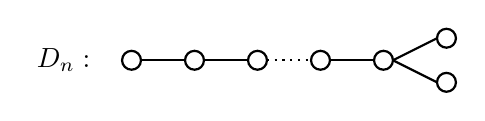
\begin{tikzpicture}[scale=.4]
\draw (-1,0) node[anchor=east]  {$D_n:$};
\foreach \x in {0,...,4}
\draw[xshift=\x cm, thick] (\x cm,0) circle (.3cm);
\draw[xshift=5 cm, thick] (5 cm, .7) circle (.3cm);
\draw[xshift=5 cm, thick] (5 cm, -.7) circle (.3cm);
\draw[thick] (0.3 cm, 0) -- +(1.4 cm, 0);
\draw[thick] (2.3 cm, 0) -- +(1.4 cm, 0);
\draw[dotted,thick] (4.3 cm, 0) -- +(1.4 cm, 0);
\draw[thick] (6.3 cm, 0) -- +(1.4 cm, 0);
\draw[thick] (8.3 cm, 0) -- +(1.4 cm, .7);
\draw[thick] (8.3 cm, 0) -- +(1.4 cm, -.7);
\end{tikzpicture}

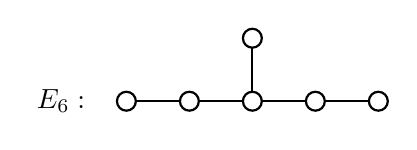
\begin{tikzpicture}[scale=.4]
\draw (-1,0) node[anchor=east]  {$E_6:$};
\foreach \x in {0,...,4}
\draw[thick,xshift=\x cm] (\x cm,0) circle (3 mm);
\foreach \y in {0,...,3}
\draw[thick,xshift=\y cm] (\y cm,0) ++(.3 cm, 0) -- +(14 mm,0);
\draw[thick] (4 cm, 2 cm) circle (3 mm);
\draw[thick] (4 cm, 3mm) -- +(0, 1.4 cm);
\end{tikzpicture}

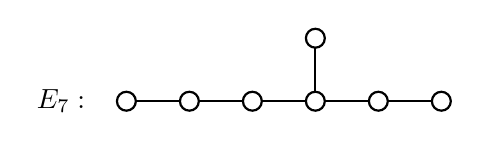
\begin{tikzpicture}[scale=.4]
\draw (-1,0) node[anchor=east]  {$E_7:$};
\foreach \x in {0,...,5}
\draw[thick,xshift=\x cm] (\x cm,0) circle (3 mm);
\foreach \y in {0,...,4}
\draw[thick,xshift=\y cm] (\y cm,0) ++(.3 cm, 0) -- +(14 mm,0);
\draw[thick] (6 cm,2 cm) circle (3 mm);
\draw[thick] (6 cm, 3mm) -- +(0, 1.4 cm);
\end{tikzpicture}

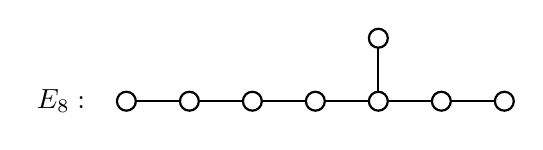
\begin{tikzpicture}[scale=.4]
\draw (-1,0) node[anchor=east]  {$E_8:$};
\foreach \x in {0,...,6}
\draw[thick,xshift=\x cm] (\x cm,0) circle (3 mm);
\foreach \y in {0,...,5}
\draw[thick,xshift=\y cm] (\y cm,0) ++(.3 cm, 0) -- +(14 mm,0);
\draw[thick] (8 cm,2 cm) circle (3 mm);
\draw[thick] (8 cm, 3mm) -- +(0, 1.4 cm);
\end{tikzpicture}

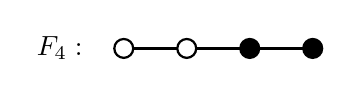
\begin{tikzpicture}[scale=.4]
\draw (-1,0) node[anchor=east] {$F_4:$};
\foreach \x in {0,...,1}
\draw[thick, xshift=\x cm] (\x cm, 0) circle (3 mm);
\foreach \x in {2,...,3}
\draw[thick, xshift=\x cm, fill=black] (\x cm, 0) circle (3 mm);
\foreach \y in {0,...,2}
\draw[thick, xshift=\y cm] (\y cm, 0) ++(.3 cm, 0) -- +(14 mm, 0);
\end{tikzpicture}

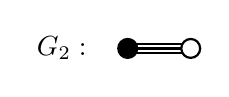
\begin{tikzpicture}[scale=.4]
\draw (-1,0) node[anchor=east]  {$G_2:$};
\draw[thick, fill=black] (0 ,0) circle (.3 cm);
\draw[thick] (2 cm,0) circle (.3 cm);
\draw[thick] (30: 3mm) -- +(1.5 cm, 0);
\draw[thick] (0: 3 mm) -- +(1.4 cm, 0);
\draw[thick] (-30: 3 mm) -- +(1.5 cm, 0);
\end{tikzpicture}

\section{Cartan Matrix}

The matrix of Cartan integers for root systems of rank 2, defined by
\begin{align*}
\left(\begin{matrix}\langle \alpha, \alpha\rangle & \langle \alpha, \beta \rangle \\ \langle \beta, \alpha \rangle & \langle \beta, \beta \rangle\end{matrix}\right).
\end{align*}
If the roots are of different length then $\alpha$ is the shorter root.

\begin{align*}
	A_1\times A_1:&\left(\begin{array}{rr}2 & 0\\0 & 2\end{array}\right) &B_2:&\left(\begin{array}{rr}2 & -1\\-2 & 2\end{array}\right) \\
	A_2:&\left(\begin{array}{rr}2 & -1\\-1 & 2\end{array}\right) &G_2:&\left(\begin{array}{rr}2 & -1\\-3 & 2\end{array}\right).
\end{align*}

\section{Rank 2 Root System Diagrams}

$A_1\times A_1:$
\begin{center}
\begin{tikzpicture}[>=latex, scale=1.2]
\pgfmathsetmacro\ax{2}
\pgfmathsetmacro\ay{0}
\pgfmathsetmacro\bx{0}
\pgfmathsetmacro\by{2}
\draw[red,->] (0,0) -- (\ax,\ay) node[right] {\(\alpha\)};
\draw[red,->] (0,0) -- (\bx,\by) node[above] {\(\beta\)};
\draw[->] (0,0) -- (-\ax,-\ay) node[left] {\(-\alpha\)};
\draw[->] (0,0) -- (-\bx,-\by) node[below] {\(-\beta\)};
\end{tikzpicture}
\end{center}

$A_2:$ 
\begin{center}
\begin{tikzpicture}[>=latex, scale=1.2]
\pgfmathsetmacro\ax{2}
\pgfmathsetmacro\ay{0}
\pgfmathsetmacro\bx{2 * cos(120)}
\pgfmathsetmacro\by{2 * sin(120)}
\draw[red,->] (0,0) -- (\ax,\ay) node[right] {\(\alpha\)};
\draw[red,->] (0,0) -- (\bx,\by) node[above left] {\(\beta\)};
\draw[->] (0,0) -- (-\ax,-\ay) node[left] {\(-\alpha\)};
\draw[->] (0,0) -- (-\bx,-\by) node[below right] {\(-\beta\)};
\draw[->] (0,0) -- (\ax + \bx,\ay + \by) node[above right] {\(\alpha+\beta\)};
\draw[->] (0,0) -- (-\ax - \bx,-\ay - \by) node[below left] {\(-\alpha-\beta\)};
\end{tikzpicture}
\end{center}

$B_2:$
\begin{center}
\begin{tikzpicture}[>=latex, scale=1.2]
\pgfmathsetmacro\ax{2}
\pgfmathsetmacro\ay{0}
\pgfmathsetmacro\bx{-2}
\pgfmathsetmacro\by{2}
\draw[red,->] (0,0) -- (\ax,\ay) node[right] {\(\alpha\)};
\draw[red,->] (0,0) -- (\bx,\by) node[above left] {\(\beta\)};
\draw[->] (0,0) -- (-\ax,-\ay) node[left] {\(-\alpha\)};
\draw[->] (0,0) -- (-\bx,-\by) node[below right] {\(-\beta\)};
\draw[->] (0,0) -- (\ax + \bx,\ay + \by) node[above] {\(\alpha+\beta\)};
\draw[->] (0,0) -- (-\ax - \bx,-\ay - \by) node[below] {\(-\alpha-\beta\)};
\draw[->] (0,0) -- (2*\ax + \bx,2*\ay + \by) node[above right] {\(2\alpha+\beta\)};
\draw[->] (0,0) -- (-2*\ax - \bx,-2*\ay - \by) node[below left] {\(-2\alpha-\beta\)};
\end{tikzpicture}
\end{center}

$G_2:$ 
\begin{center}
\begin{tikzpicture}[>=latex, scale=1.2]
\pgfmathsetmacro\ax{2}
\pgfmathsetmacro\ay{0}
\pgfmathsetmacro\abx{2 * cos(120)}
\pgfmathsetmacro\aby{2 * sin(120)}
\draw[red,->] (0,0) -- (\ax,\ay) node[below right] {\(\alpha\)};
\draw[red,->] (0,0) -- (-\ax + \abx,-\ay + \aby) node[above] {\(\beta\)};
\draw[->] (0,0) -- (-\ax,-\ay) node[below left] {\(-\alpha\)};
\draw[->] (0,0) -- (\ax - \abx,\ay - \aby) node[below] {\(-\beta\)};
\draw[->] (0,0) -- (\abx,\aby) node[above] {\(\alpha+\beta\)};
\draw[->] (0,0) -- (-\abx,-\aby) node[below] {\(-\alpha-\beta\)};
\draw[->] (0,0) -- (\ax + \abx,\ay + \aby) node[above] {\(2\alpha+\beta\)};
\draw[->] (0,0) -- (-\ax-\abx,-\ay-\aby) node[below] {\(-2\alpha-\beta\)};
\draw[->] (0,0) -- (2*\ax + \abx,2*\ay + \aby) node[above] {\(3\alpha+\beta\)};
\draw[->] (0,0) -- (-2*\ax - \abx,-2*\ay - \aby) node[below] {\(-3\alpha-\beta\)};
\draw[->] (0,0) -- (\ax + 2*\abx,\ay + 2*\aby) node[above] {\(3\alpha+2\beta\)};
\draw[->] (0,0) -- (-\ax - 2*\abx,-\ay - 2*\aby) node[below] {\(-3\alpha-2\beta\)};
\end{tikzpicture}
\end{center}
